\subsection{FRFs of the system due to a multiple point force}
\label{subsec:FRFs_of_the_system_due_to_multiple_point_force}

The next step is to observe the behavior of the structure when multiple forces are applied to it.

As we have said in the previous section, even if the FRF given information about a single input and a single output, we can still use it to understand how the structure behaves when multiple forces are applied to it and study the structural response at different coordinates.

For the sake of simplicity, we will consider a structure with $2$ excitation points at $x_k = [0.3 \quad 0.9]m$ and $3$ output points at $x_j = [0.2 \quad 0.8 \quad 1.2]m$.

A graphical representation of the considered situation can be seen in Figure \ref{fig:beam_multi_point_force}.

\begin{figure}[H]
    \centering
    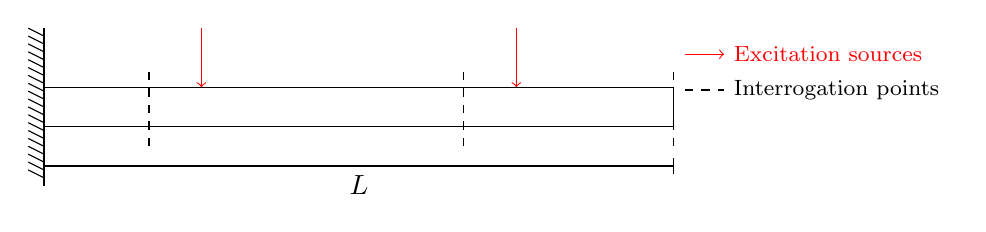
\begin{tikzpicture}[xscale=1, yscale=0.5]

        \draw (0,-0.5) rectangle (8, 0.5);
        \draw[|-|] (0, -1.5) -- (8, -1.5) node[midway, below]{$L$};

        \draw (0, -2) -- (0,  2);

        \foreach \y in {-1.8, -1.6, ..., 1.8}
        \draw (0, \y) -- ++(-0.2, +0.2);

        \foreach \x in {0.2, 0.8, 1.2}
        \draw[dashed] (\x * 8/1.2, -1.0) -- ++(0.0, +2.0);

        \foreach \x in {0.3, 0.9}
        \draw[<-, red] (\x * 8/1.2, 0.5) -- ++(0.0, +1.5);

        % Add legend
        \node [matrix, font = \footnotesize, below right, row sep = 0cm] at (current bounding box.north east)
        {
            \draw[->, red] (0, 0) -- ++(0.5, 0) node[right, red] {Excitation sources}; \\
            \draw[dashed, black] (0, 0) -- ++(0.5, 0) node[right, black] {Interrogation points}; \\
        };

    \end{tikzpicture}
    \caption{Analyzed situation: multiple inputs, multiple outputs}
    \label{fig:beam_multi_point_force}
\end{figure}

Similar reasoning as before can be done about the expected result of this type of analysis in terms of number of FRFs to be computed and the information that can be extracted from them.

Moreover, given that we are now dealing with a multi-input system, the actual displacement of the structure at a specific coordinate will be the result of the superposition of the displacements due to each excitation force.

Before proceeding with the visualization of the actual FRFs, it's important to stress that what we are actually "superposing" are the complex FRFs, not only their modules.
This means that the phase information is also taken into account when computing the total response of the structure (which indeed depends on the phase of the input forces).

To better understand this aspect, we can move on a complex plane and consider the output of a generic system due to two different input forces $F_1 = F_{1,0} \sin(\omega_1 t + \phi_1)$ and $F_2 = F_{2,0} \sin(\omega_2 t + \phi_2)$.

\begin{figure}[H]
    \centering
    \begin{tikzpicture}

        \coordinate (O) at (0, 0);
        \coordinate (A) at (2, 1);
        \coordinate (B) at (-3, 1);
        \coordinate (C) at (3, -2);
        \coordinate (D) at (-2, 4);

        \draw[->] (-3,0) -- (3,0) node[right] {Re};
        \draw[->] (0,-3) -- (0,3) node[above] {Im};

        \draw[->, thick, red] (O) -- (A) node[midway, above, sloped] {$F_1$};
        \draw[->, thick, red] (O) -- (B) node[midway, above, sloped] {$F_2$};
        \draw[->, thick] (O) -- (C) node[midway, above, sloped] {$FRF_1$};
        \draw[->, thick] (O) -- (D) node[midway, above, sloped] {$FRF_2$};

        \pic [draw, <-, "$\phi_{FRF1}$", angle radius = 2cm] {angle = C--O--A};
        \pic [draw, <-, "$\phi_{FRF2}$", angle radius = 1cm] {angle = D--O--B};

    \end{tikzpicture}
    \hspace{1cm}
    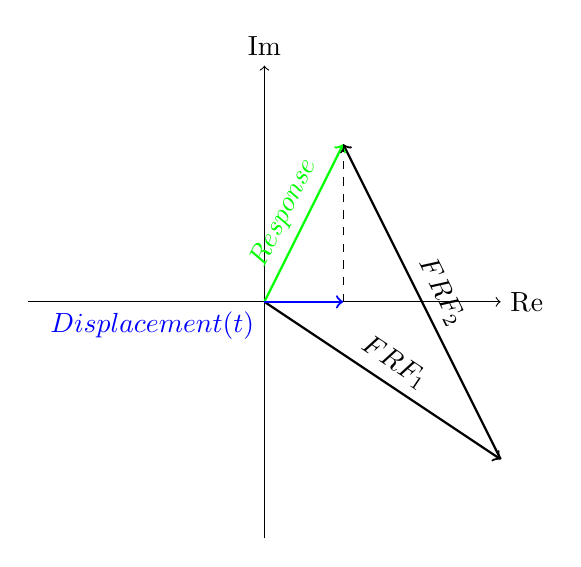
\begin{tikzpicture}

        \coordinate (O) at (0, 0);
        \coordinate (A) at (2, 1);
        \coordinate (B) at (-3, 1);
        \coordinate (C) at (3, -2);
        \coordinate (D) at (-2, 4);

        \draw[->] (-3,0) -- (3,0) node[right] {Re};
        \draw[->] (0,-3) -- (0,3) node[above] {Im};

        \draw[->, thick] (O) -- (C) node[midway, above, sloped] {$FRF_1$};
        \draw[->, thick] (C) -- ++(D) node[midway, above, sloped] {$FRF_2$};

        \draw[->, thick, green] (O) -- (1, 2) node[midway, above, sloped] {$Response$};
        \draw[dashed] (1, 0) -- (1, 2);
        \draw[->, thick, blue] (O) -- (1, 0) node[below left] at (O) {$\text{Displacement}(t)$};



    \end{tikzpicture}
    \caption{Complex plane representation of the FRFs of the system due to multiple input forces and the actual displacement of the output/interrogation point.}
    \label{fig:complex_plane_representation}
\end{figure}

As is clearly see in Figure \ref{fig:complex_plane_representation}, the actual displacement of the output point can in some cases (or better for some period of time) be definitely lower than the sum of just the absolute modules of the FRFs.
Notice, however, that if the two acting forces have different periods (frequencies), there also be some time instants where the actual displacement is effectively the sum of the two modules of the FRFs.
So in general, if we are just interested in the maximum displacement of the output point, we can simply sum the modules of all the FRFs due to the different input forces.

If we go back and considering again the situation represented in Figure \ref{fig:beam_multi_point_force}, we obtain the module and phase plots reported in Figure \ref{fig:FRFs_multi_point_force}.

\begin{figure}[H]
    \centering
    \includegraphics[width=\textwidth]{img/MATLAB/Part_A/Experimental_FRF_MIMO.png}
    \caption{FRFs of the system due to a couple of point force. Each color in the plot represents the FRF of the structure at a specific output coordinate.}
    \label{fig:FRFs_multi_point_force}
\end{figure}
